Una comunicación establecida entre dos partes, Alice y Bob, con el objetivo de obtener confidencialidad en un canal inseguro, puede expresarse mediante el siguiente diagrama:

\begin{center}
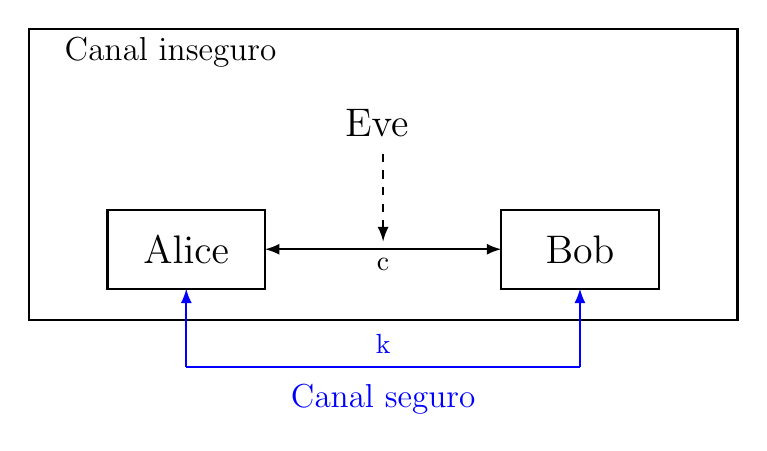
\begin{tikzpicture}[>=latex]

    % 1. Caja grande exterior (canal inseguro)
    \draw[thick] (-2, -1.2) rectangle (7, 2.5);
    \node at (-0.2, 2.2) {\large Canal inseguro};

    % 2. Caja A (Alice) - más arriba
    \draw[thick] (-1, -0.8) rectangle (1, 0.2);
    \node at (0, -0.3) {\Large Alice};

    % 3. Caja B (Bob) - más arriba
    \draw[thick] (4, -0.8) rectangle (6, 0.2);
    \node at (5, -0.3) {\Large Bob};

    % 4. Caja E (Eve) - abajo
    \node at (2.42, 1.3) {\Large Eve};

    % 4. Flecha del mensaje
    \draw[<->, thick] (1, -0.3) -- (4, -0.3);
    \node at (2.5, -0.5) {c};
    
    % 5. Flecha de Eve
    \draw[<-, dashed, thick] (2.5, -0.2) -- (2.5, 1);

    % 6 canal seguro
    \draw[<-,thick, blue] (0, -0.8) -- (0, -1.8);
    \draw[-, thick, blue] (0, -1.8) -- (5, -1.8);
    \draw[->, thick, blue] (5, -1.8) -- (5, -0.8);
    \node at (2.5, -2.2) [blue] {\large Canal seguro};
    \node at (2.5, -1.5) [blue] {k};
    
\end{tikzpicture}
\end{center}

\noindent Donde Alice y Bob comparten una clave secreta \textit{k} a través de un canal seguro, la cual utilizan para encriptar mensajes, \textit{m}, y enviarlos por el canal inseguro en forma de  texto cifrado, $c$. Para descifrar $c$ se utiliza la misma clave \textit{k}, obteniendo así el mensaje original \textit{m}. A priori, Eve no puede obtener información acerca de \textit{m}, pues solo conoce \textit{c}. A pesar de ello, se supone que Eve es una entidad con una gran cantidad de medios e intentará romper el cifrado, para así obtener información acerca de \textit{m} (la disciplina encargada de estudiar vulnerabilidades en los algoritmos de encriptación y descifrado se llama criptoanálisis). En general, el proceso mediante el cual se encripta y se descifra son conocidos públicamente, de tal forma que solamente aquellos con conocimiento de la clave puedan obtener información acerca del mensaje.

La nomenclatura ``clave simétrica'' proviene de que tanto Alice como Bob utilizan la misma clave \textit{k} para encriptar y descifrar. De manera formal, se definen los siguientes elementos:
    \begin{enumerate}[label={--}]
        \item Sea \textit{M} el conjunto de todas las cadenas que se pueden obtener utilizando un alfabeto $\mathcal{A}$. Un elemento \textit{m} de \textit{M} se denomina \textit{texto claro}, y es la información que se pretende enviar.
        \item Sea \textit{C} el conjunto de todas las cadenas que se pueden obtener utilizando un alfabeto $\mathcal{B}$. Un elemento \textit{c} de \textit{C} se denomina \textit{texto cifrado}, y es la información que se envía a través del canal inseguro. De forma general, será $\mathcal{B} = \mathcal{A}$.
        \item Sea \textit{K} el conjunto de claves, \textit{k}, que se pueden utilizar para encriptar/descifrar.
        \item $\forall k\in K$ sean $E_k $ y $ D_k$ los conjuntos de funciones $e_k: M \to C$ y $d_k: C \to M$ que transforman texto claro en texto cifrado (Encriptan), y texto cifrado en texto claro (Desencriptan), cumpliéndose que $d_k(e_k(m)) = m$, es decir, que encriptar y luego desencriptar un mensaje dé como resultado el mismo mensaje. A las $e_k$ se les llama funciones encriptadoras, mientras que a las $d_k$ funciones desencriptadoras.
    \end{enumerate}

\begin{ejs}\label{ej:flujo_bloque_xor}
    \item Sean \textit{M} =  \textit{C} = \textit{K} el conjunto de todas las cadenas posibles definidas en el alfabeto binario. Dado un mensaje $m\in M$, se toma una clave $k\in K$ de igual número de bits y se define $e_k \in E_k$ como $e_k(m) = m \oplus k = c$, donde $m \oplus k$ es la operación XOR bit a bit de ambas cadenas, definida como:
    \[
    \ 0 \oplus 0 = 0; \ 1 \oplus 0 = 1; \ 0 \oplus 1 = 1; \ 1 \oplus 1 = 0.
    \]
   La función $d_k\in D_k$ es la operación inversa de $e_k$: $d_k(c) = c \oplus k = m$. De esta forma, si Alice quiere enviar $m = 01001000$ a Bob usando la clave $k = 00101110$, encriptará $m$ mediante $e_k$: $e_k(m) = 01001000 \oplus 00101110 = 01100110 = c$, enviando $c$ a través del canal inseguro, y Bob desencriptará $c$ mediante $d_k$ obteniendo $m$. El proceso se muestra en la tabla \ref{tab:flujo_ejemplo1}.
    
\begin{table}[H]
    \centering
    \setlength{\tabcolsep}{12pt}
    \begin{tabular}{cccc}
    \toprule
    $m$ & $k$ & $m \oplus k = c$ & $c \oplus k = m$ \\
    \midrule
     0 & 0 & $0 \oplus 0 = 0$ & $0 \oplus 0 = 0$ \\
     1 & 0 & $1 \oplus 0 = 1$ & $1 \oplus 0 = 1$ \\
     0 & 1 & $0 \oplus 1 = 1$ & $1 \oplus 1 = 0$ \\
     0 & 0 & $0 \oplus 0 = 0$ & $0 \oplus 0 = 0$ \\
     1 & 1 & $1 \oplus 1 = 0$ & $0 \oplus 1 = 1$ \\
     0 & 1 & $0 \oplus 1 = 1$ & $1 \oplus 1 = 0$ \\
     0 & 1 & $0 \oplus 1 = 1$ & $1 \oplus 1 = 0$ \\
     0 & 0 & $0 \oplus 0 = 0$ & $0 \oplus 0 = 0$ \\
    \bottomrule
    \end{tabular}
\caption{Encriptación bit a bit.}
\label{tab:flujo_ejemplo1}
\end{table}
Si luego Bob respondiera a Alice con $m' = 01101111$ utilizando la misma clave, enviando $c' = 01000001$, Eve podría obtener información acerca del mensaje sumando $c$ y $c'$, pues se tiene que $c \oplus c' = m \oplus k \oplus m' \oplus k = m \oplus m'$, y aunque no pueda inferir directamente $m$ o $m'$ a partir de su suma en este caso, puede reducir el marco de trabajo si sabe que se han enviado letras del abecedario: $m = H$ y $m'=o$. En general, reutilizar una misma clave para distintos mensajes puede permitir a un tercero obtener información acerca de los mensajes, por lo que se considera mala praxis.

    \item Tomando de nuevo $M,C$ definidos en el alfabeto binario, $K = \{0,1,2,3\}$, la función encriptadora $e_k(m)$, que toma bloques de 4 bits de $m$ y los permuta $k$ unidades a la derecha de forma que el extremo pasa al otro extremo, y la función desencriptadora, que toma bloques de 4 bits de $m$ y los permuta $k$ unidades a la izquierda de la misma forma. Tomando $m = 01001000$ y $k = 3$, se tiene $c = 10000001$, tal y como puede verse en la Tabla \ref{tab:bloque_ejemplo1}.

    \begin{table}[H]
    \centering
    \setlength{\tabcolsep}{12pt}
    \begin{tabular}{ccc}
    \toprule
    $m$ & $e_3(m) = c$ & $d_3(c) = m$ \\
    \midrule
     0100 &$0100 \to 1000$& $1000 \to 0100$ \\
     1000 &$1000 \to 0001$& $0001 \to 1000$ \\
    \bottomrule
    \end{tabular}
\caption{Encriptación por bloques de 4 bits.}
\label{tab:bloque_ejemplo1}
\end{table}
Si el mensaje $m$ estuviera formado por varios bloques iguales, los bloques correspondientes del texto cifrado $c$ serían de nuevo iguales, y un atacante obtendría por lo tanto información del mensaje original (que se repite cierta información dentro del mensaje). Para evitarlo, se utilizan distintas estrategias, como puede ser sumar el resultado del bloque anterior al nuevo bloque antes de realizar las operaciones de bloque. Si en el ejemplo anterior fuera $m = 10001000$, con bloques $m_1 = m_2 = 1000$, se tendría que $c_1 = 0001$, mientras que para obtener $c_2$, primero se suma $m_2 \oplus c1 = 1001$, y luego se permuta 3 veces a la derecha, obteniendo $c_2 = 0011$, resultando dos bloques diferentes a partir de dos bloques iguales. Para desencriptar, el primer bloque se obtiene haciendo $d_3(c_1) = 1000$; mientras que el segundo bloque se desencripta sumando $c_1$ después de aplicar $d_3$, es decir,  $m_2 = c_1 \oplus d_3(c_2) = 0001 \oplus 1001 = 1000$.

\end{ejs}
Los ejemplos anteriores ilustran los dos tipos de cifrado simétrico utilizados en criptografía: el cifrado de flujo y el cifrado por bloques. El cifrado de flujo opera bit a bit, mientras que el cifrado por bloques realiza las mismas operaciones en cada bloque.
